\documentclass{article}

% packages
\usepackage{amsmath, amsthm, thmtools, amsfonts, amssymb, luacode, catchfile, tikzducks, hyperref, ifthen}
\ifcsname c@kobocompile\endcsname
	\usepackage[a5paper, total={1072pt, 1448pt}, margin=10pt, includeheadfoot]{geometry} % set page margins
\else
	\usepackage[a4paper, margin=50pt, includeheadfoot]{geometry}
\fi
\usepackage[shortlabels]{enumitem}
\usepackage[skip=3pt, indent=0pt]{parskip}

% language
\usepackage[bidi=basic, layout=tabular, provide=*]{babel}
\ifcsname c@english\endcsname
	\babelprovide[main, import]{english}
\else
	\babelprovide[main, import]{hebrew}
	\babelprovide{rl}
\fi
%\babelfont{rm}{Libertinus Serif}
\babelfont{rm}[Renderer=Harfbuzz]{Libertinus Serif}
\babelfont{sf}{Libertinus Sans}
\babelfont{tt}{Libertinus Mono}

% style
\AddToHook{cmd/section/before}{\clearpage}	% Add line break before section
\linespread{1.3}
\setcounter{secnumdepth}{0}		% Remove default number tags from sections, this won't do well with theorems
\AtBeginDocument{\setlength{\belowdisplayskip}{3pt}}
\AtBeginDocument{\setlength{\abovedisplayskip}{3pt}}
\graphicspath{ {../images/} }

% operators
\DeclareMathOperator\cis{cis}
\DeclareMathOperator\Sp{Sp}
\DeclareMathOperator\tr{tr}
\DeclareMathOperator\im{Im}
\DeclareMathOperator\re{Re}
\DeclareMathOperator\diag{diag}
\DeclareMathOperator*\lowlim{\underline{lim}}
\DeclareMathOperator*\uplim{\overline{lim}}
\DeclareMathOperator\rng{rng}
\DeclareMathOperator\Sym{Sym}
\DeclareMathOperator\Arg{Arg}
\DeclareMathOperator\Log{Log}
\DeclareMathOperator\dom{dom}
\DeclareMathOperator\supp{Supp}
\DeclareMathOperator\var{Var}
\DeclareMathOperator\cov{Cov}

% commands
%\renewcommand\qedsymbol{\textbf{מש''ל}}
%\renewcommand\qedsymbol{\fbox{\emoji{lizard}}}
\newcommand{\Aa}[0]{\mathcal{A}}
\newcommand{\Bb}[0]{\mathcal{B}}
\newcommand{\CC}[0]{\mathbb{C}}
\newcommand{\Cc}[0]{\mathcal{C}}
\newcommand{\EE}[0]{\mathbb{E}}
\newcommand{\FF}[0]{\mathbb{F}}
\newcommand{\Ff}[0]{\mathcal{F}}
\newcommand{\Ii}[0]{\mathcal{I}}
\newcommand{\Gg}[0]{\mathcal{G}}
\newcommand{\Ll}[0]{\mathcal{L}}
\newcommand{\Mm}[0]{\mathcal{M}}
\newcommand{\NN}[0]{\mathbb{N}}
\newcommand{\Nn}[0]{\mathcal{N}}
\newcommand{\PP}[0]{\mathbb{P}}
\newcommand{\Pp}[0]{\mathcal{P}}
\newcommand{\QQ}[0]{\mathbb{Q}}
\newcommand{\RR}[0]{\mathbb{R}}
\newcommand{\Rr}[0]{\mathcal{R}}
\newcommand{\Ss}[0]{\mathcal{S}}
\newcommand{\TT}[0]{\mathbb{T}}
\newcommand{\Uu}[0]{\mathcal{U}}
\newcommand{\Vv}[0]{\mathcal{V}}
\newcommand{\Ww}[0]{\mathcal{W}}
\newcommand{\ZZ}[0]{\mathbb{Z}}
\newcommand{\acts}[0]{\circlearrowright}
\newcommand{\explain}[2] {
	\begin{flalign*}
		 && \text{#2} && \text{#1}
	\end{flalign*}
}
\newcommand{\maketitleprint}[0]{ \begin{center}
	%\begin{tikzpicture}[scale=3]
	%	\duck[graduate=gray!20!black, tassel=red!70!black]
	%\end{tikzpicture}	
	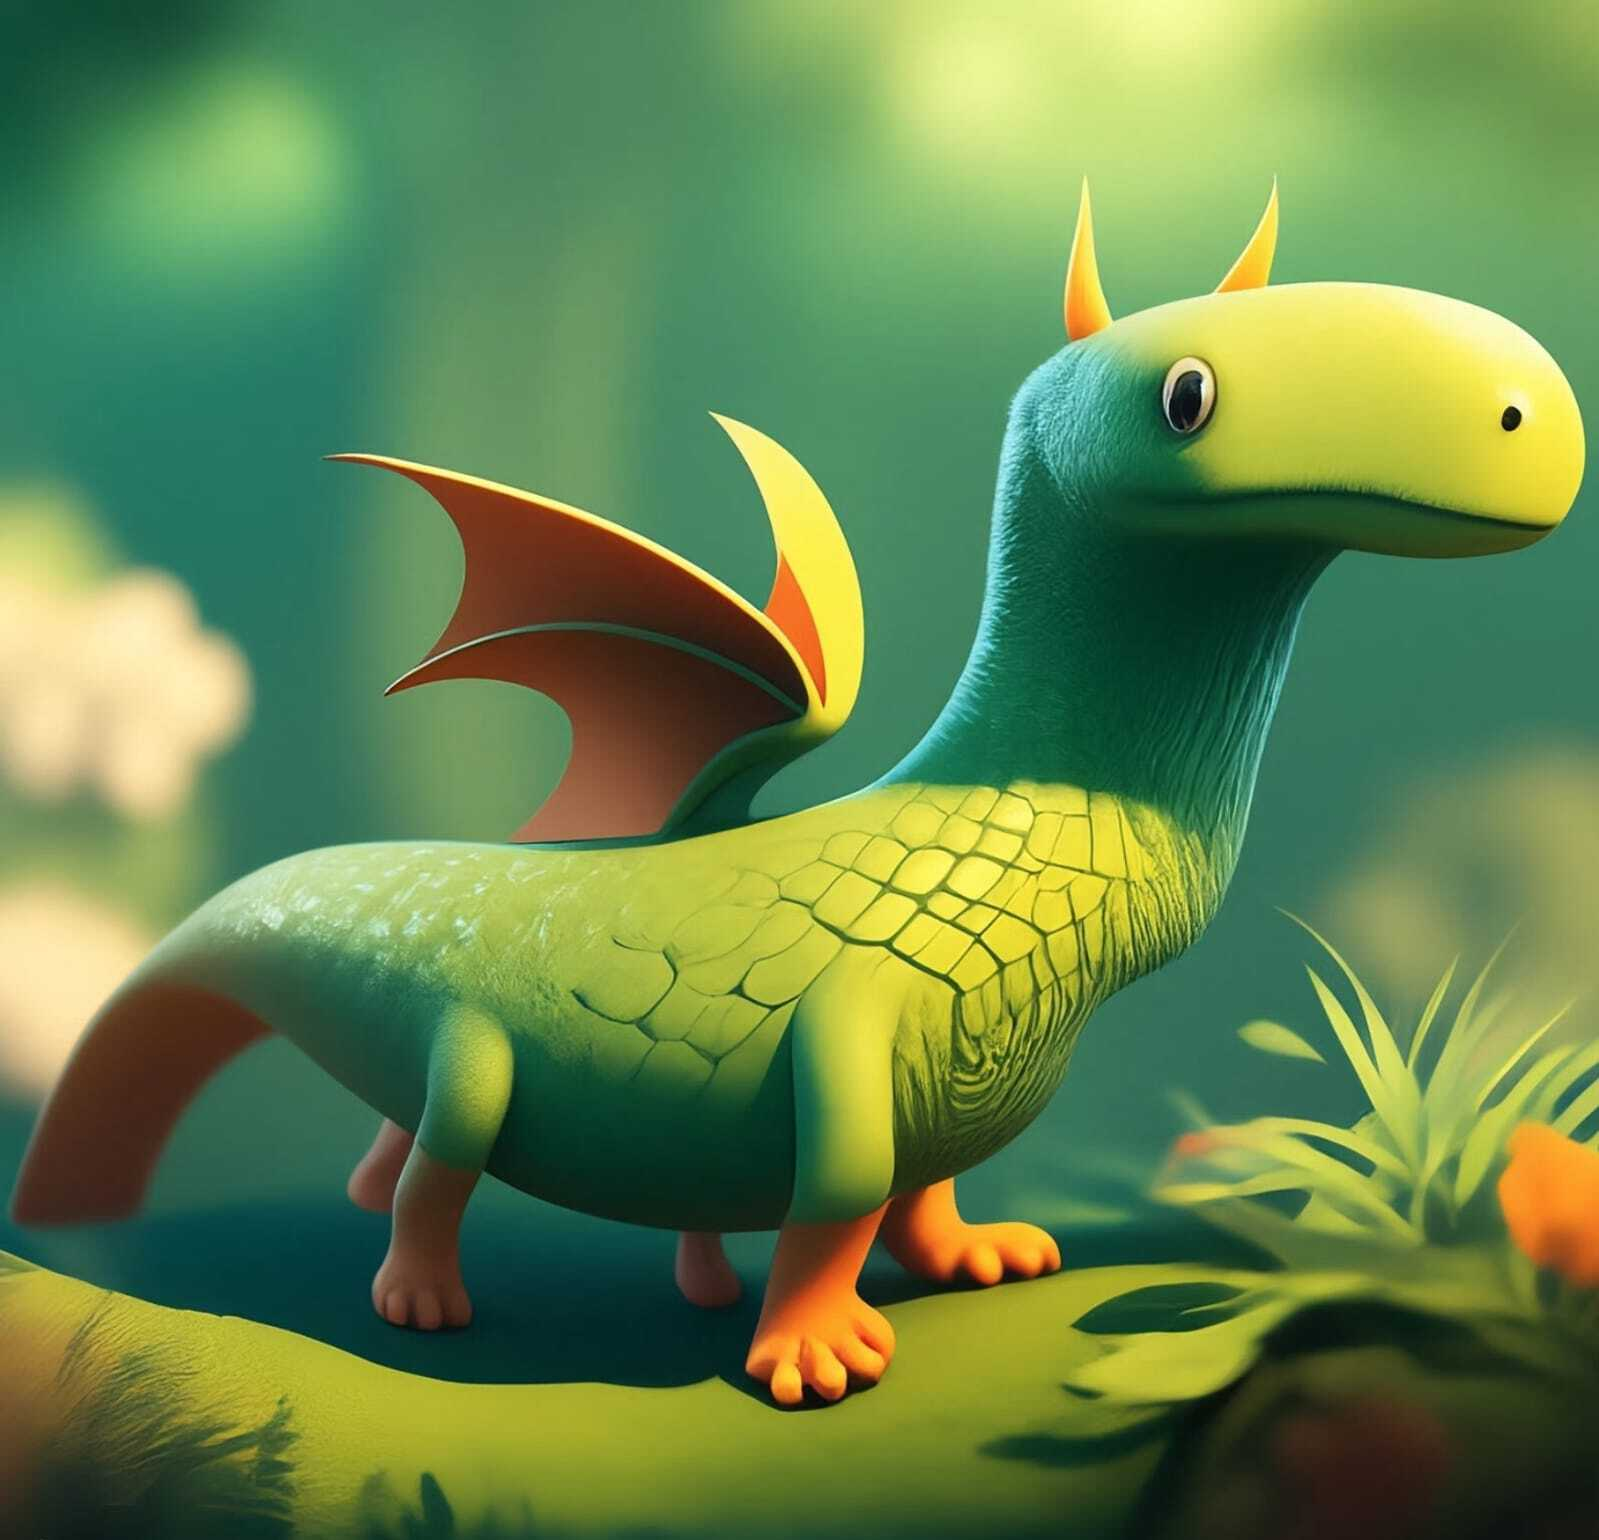
\includegraphics[width=6cm]{cover}
\end{center}
}

% theorem commands
\newtheoremstyle{c_remark}
	{}	% Space above
	{}	% Space below
	{}% Body font
	{}	% Indent amount
	{\bfseries}	% Theorem head font
	{}	% Punctuation after theorem head
	{.5em}	% Space after theorem head
	{\thmname{#1}\thmnumber{ #2}\thmnote{ \normalfont{\text{(#3)}}}}	% head content
\newtheoremstyle{c_definition}
	{3pt}	% Space above
	{3pt}	% Space below
	{}% Body font
	{}	% Indent amount
	{\bfseries}	% Theorem head font
	{}	% Punctuation after theorem head
	{.5em}	% Space after theorem head
	{\thmname{#1}\thmnumber{ #2}\thmnote{ \normalfont{\text{(#3)}}}}	% head content
\newtheoremstyle{c_plain}
	{3pt}	% Space above
	{3pt}	% Space below
	{\itshape}% Body font
	{}	% Indent amount
	{\bfseries}	% Theorem head font
	{}	% Punctuation after theorem head
	{.5em}	% Space after theorem head
	{\thmname{#1}\thmnumber{ #2}\thmnote{ \text{(#3)}}}	% head content

\ifcsname c@english\endcsname
	\theoremstyle{plain}
	\newtheorem{theorem}{Theorem}[section]
	\newtheorem{lemma}[theorem]{Lemma}
	\newtheorem{proposition}[theorem]{Proposition}
	\newtheorem*{proposition*}{Proposition}
	%\newtheorem{corollary}[theorem]{אין חלופה עברית}

	\theoremstyle{definition}
	\newtheorem{definition}[theorem]{Definition}
	\newtheorem*{definition*}{Definition}
	\newtheorem{example}{Example}[section]
	\newtheorem{exercise}{Exercise}[section]

	\theoremstyle{remark}
	\newtheorem*{remark}{Remark}
	\newtheorem*{solution}{Solution}
	\newtheorem{conclusion}[theorem]{Conclusion}
	\newtheorem{notation}[theorem]{Notation}
\else
	\theoremstyle{c_plain}
	\newtheorem{theorem}{משפט}[section]
	\newtheorem{lemma}[theorem]{למה}
	\newtheorem{proposition}[theorem]{טענה}
	\newtheorem*{proposition*}{טענה}
	%\newtheorem{corollary}[theorem]{אין חלופה עברית}

	\theoremstyle{c_definition}
	\newtheorem{definition}[theorem]{הגדרה}
	\newtheorem*{definition*}{הגדרה}
	\newtheorem{example}{דוגמה}[section]
	\newtheorem{exercise}{תרגיל}[section]

	\theoremstyle{c_remark}
	\newtheorem*{remark}{הערה}
	\newtheorem*{solution}{פתרון}
	\newtheorem{conclusion}[theorem]{מסקנה}
	\newtheorem{notation}[theorem]{סימון}
\fi

% Questions related commands
\newcounter{question}
\setcounter{question}{1}
\newcounter{sub_question}
\setcounter{sub_question}{1}

\ifcsname c@english\endcsname
	\newcommand{\question}[1][0]{
		\ifthenelse{#1 = 0}{}{\setcounter{question}{#1}}
		\section{Question \arabic{question}}
		\addtocounter{question}{1}
		\setcounter{sub_question}{1}
	}

	\newcommand{\subquestion}[1][0]{
		\ifthenelse{#1 = 0}{}{\setcounter{sub_question}{#1}}
		\subsection{Part \alph{sub_question}}
		\addtocounter{sub_question}{1}
	}
\else
	\newcommand{\question}[1][0]{
		\ifthenelse{#1 = 0}{}{\setcounter{question}{#1}}
		\section{שאלה \arabic{question}}
		\addtocounter{question}{1}
		\setcounter{sub_question}{1}
	}

	\newcommand{\subquestion}[1][0]{
		\ifthenelse{#1 = 0}{}{\setcounter{sub_question}{#1}}
		\subsection{סעיף \localecounter{letters.gershayim}{sub_question}}
		\addtocounter{sub_question}{1}
	}
\fi

% import lua and start of document
\directlua{common = require ('../common')}

\GetEnv{AUTHOR}

% headers
\author{\AUTHOR}
\date\today

\title{פתרון מטלה 07 --- מבנים אלגבריים (2), 80446}

\begin{document}
\maketitle
\maketitleprint[red]

\question{}
נסמן $F = \QQ(s)$ ויהי $K$ שדה הפיצול של $x^n - s \in F[x]$. \\
נראה ש־$\aut(K / F) \simeq {(\ZZ / n \ZZ)}^\times \ltimes_{\theta} (\ZZ / n \ZZ)$, כאשר,
\[
	\theta : {(\ZZ / n \ZZ)}^\times \to \aut(\ZZ / n \ZZ),
	\qquad
	\theta(k)(n) = k n
\]
\begin{proof}
	בתרגול ראינו כי מכפלה חצי־ישרה זו היא איזומורפית לחבורת הפונקציות,
	\[
		G = \{ f : \ZZ / n \ZZ \to \ZZ / n \ZZ \mid \exists c, d,\ \forall x \in \ZZ / n \ZZ,\ f(x) = cx + d \}
	\]
	אנו נראה אם כך ש־$\aut(K / F) \simeq G$.
	%תהי $\varphi \in \aut(K / F)$, אז נגדיר $f \in G$ על־ידי $f(x) = \varphi(e)$
	בתרגול כבר ראינו כי קיים שיכון כזה, כלומר מצאנו שזהו הומומורפיזם חד־חד ערכי, ולכן עלינו רק להראות שהומומורפיזם זה הוא גם על.
	תהי $f \in G$, ונניח ש־$c, d$ קבועים כך ש־$f(x) = cx + d$.
	אנו יודעים כי $\xi_n^c \in K$ ולכן $\xi_n^m x \mapsto \xi_n^{mc + d} x^c$ הוא אוטומורפיזם תקין, כאשר ההוכחה לטענה זו זהה לזו שראינו בתרגול.
	נסמן ב־$\psi$ אוטומורפיזם זה ונקבל ש־$\aut(K / F) \ni \psi \mapsto f \in G$ בדיוק, ובכך נקבל שהומומורפיזם זה אכן על, ובהתאם הוא אוטומורפיזם.
\end{proof}

\question{}
תהי $L / \QQ$ הרחבה אלגברית נוצרת סופית.
נראה שב־$L$ יש מספר סופי של שורשי יחידה.
\begin{proof}
	נניח בשלילה שב־$L$ יש אינסוף שורשי יחידה.
	בפרט יש אינסוף שורשי יחידה פרימיטיביים, שאם לא כן יש כמות סופית של שורשי יחידה. \\
	בלי הגבלת הכלליות נוכל לבחור אינסוף שורשי יחידה פרימיטיביים מסדר ראשוני, אחרת מהעובדה שיש אינסוף שורשים פרימיטיביים נוכל לבחור מכפלות ולבודד ראשוניים.
	נסמן ${\{ \xi_{p_i} \}}_{i = 1}^\infty$ שורשי יחידה פרימיטיביים מסדר $p_i$ ראשוני כך ש־$p_i \ne p_j$ לכל $i \ne j$. \\
	ידוע כי $L / \QQ$ נוצרת סופית ולכן ישנה כמות סופית של פולינומים המגדירים את ההרחבה, אבל $\xi_{p_i}$ מעיד על הפולינום $x^{p_i} - 1$ כפולינום שניתן לפיצול בהרחבה,
	ולכן קיבלנו שיש ${\{ x^{p_i} - 1 \}}_{i = 1}^\infty$ פולינומים, בפרט כמות אינסופית, בסתירה.
\end{proof}

\question{}
יהי $K$ שדה פיצול של $x^8 - 2$ מעל $\QQ$.

\subquestion{}
נראה שניתן לזהות את $K$ עם השדה $\QQ(i)(\sqrt[8]{2}) \subseteq \CC$,
כאשר שורש מוגדר לפי הענף הראשי של השורש.
\begin{proof}
	נבחין כי $\xi_8 \sqrt[8]{2} \in K$, אבל $\xi_8 = e^{\frac{2\pi i}{8}} = \frac{1 + i}{\sqrt{2}}$.
	\[
		{(\xi_8 \sqrt[8]{2})}^2
		= i \cdot \sqrt[4]{2}
		\qquad
		{(\xi_8 \sqrt[8]{2})}^6
		= -i \cdot \sqrt[4]{2} \cdot \sqrt{2}
	\]
	ולכן בפרט גם,
	\[
		{(\xi_8 \sqrt[8]{2})}^2 - {(\xi_8 \sqrt[8]{2})}^6
		= \sqrt[4]{2} i (1 + \sqrt{2})
		\in K
	\]
	וכן,
	\[
		\frac{\sqrt[4]{2} i (1 + \sqrt{2})}{{(\xi_8 \sqrt[8]{2})}^2}
		1 + \sqrt{2} \in K
	\]
	ונסיק ש־$\sqrt{2} \in K$.
	אז גם $(1 + i) \sqrt[8]{2} \in K$, אבל באותו אופן תוך שימוש בחזקה שביעית נקבל שגם $(1 - i) \sqrt[8]{2} \in K$ ולכן $i, \sqrt[8]{2} \in K$.
	לכן $\QQ(i, \sqrt[8]{2}) \subseteq K$, אבל אנו כבר יודעים כי $\QQ(i, \sqrt[8]{2}) \supseteq K$ ממהלך ההוכחה, ולכן השדות שווים.

	נבחין כי טענה זו עד כדי אוטומורפיזם המצמיד לשורשים הפרימיטיביים שבחרנו.
\end{proof}

\subquestion{}
נראה ש־$x^8 - 2$ אי־פריק ב־$\QQ(i)$.
\begin{proof}
	נבחין כי $\QQ(i)(\sqrt[8]{2}) = \QQ(i)[x] / (x^8 - 2)$ הוא שדה ולכן בפרט $x^8 - 2$ אי־פריק ב־$\QQ(i)$.
	זאת ישירות מהטענה כי $\sqrt[8]{2}$ הוא האיבר שהפולינום המינימלי שלו הוא $x^8 - 2$.
\end{proof}

\subquestion{}
נוכיח שעבור $\varepsilon \in \{-1, 1\}$ ולכל שורש $z$ של $x^8 - 2$ קיים אוטומורפיזם של $K$ כך ש־$i \mapsto \varepsilon i$ ו־$\sqrt[8]{2} \mapsto z$
\begin{proof}
	נניח ש־$z = \sqrt[8]{2} \xi_8^m$ עבור $0 \le m < n$.
	ראינו כי $\aut(\QQ(\sqrt[8]{2}, i) / \QQ) \simeq G$ עבור $G$ משאלה 1. \\
	נגדיר את הפונקציה $f : \ZZ / 8\ZZ \to \ZZ / 8\ZZ$ על־ידי,
	\[
		f(x) = (2 + \varepsilon) x + m
	\]
	ולכן משאלה 1 קיים אוטומורפיזם $\iota \in \aut(\QQ(\sqrt[8]{2}, i) / \QQ)$ כך שמתקיים,
	\[
		\iota(\sqrt[8]{2})
		= \xi_8^{(2 + \varepsilon) \cdot 0 + m} \sqrt[8]{2}
		= z
	\]
	בנוסף גם,
	\[
		\iota(i)
		= \iota(\xi_8^2)
		= \xi_8^{(2 - \varepsilon) \cdot 2}
		= -1 \cdot \xi_8^{-2\varepsilon}
		= \varepsilon i
	\]
	ומצאנו אוטומורפיזם המקיים את הרצוי.
\end{proof}

\subquestion{}
נמצא שיכון של $\aut(K / \QQ)$ אל תוך החבורה המתוארת בסעיף א' ונמצא את תמונתה.
\begin{solution}
	נבחין כי ${(\ZZ / 8 \ZZ)}^\times = \{1, 3, 5, 7\}$ ולכן השיכון הוא לתוך $\{1, 3, 5, 7\} \ltimes_{\theta} (\ZZ / 8\ZZ)$ על־ידי אותו שיכון המתואר בסעיף הקודם.
\end{solution}

\question{}
יהי $p$ ראשוני ונסמן $K = \overline{\FF_p}(s, t)$.

\subquestion{}
נראה ש־$[K^{1 / p} : K] = p^2$.
\begin{proof}
	נבחין כי לכל $x \in \overline{\FF_p}$ יש שורש $p$ שכן $\overline{\FF_p}$ שדה מושלם.
	בנוסף אנו יודעים כי $s, t \in K$ וכי קיימים $\alpha, \beta \in K^{1 / p}$ כך ש־$s = \alpha^p, t = \beta^p$.
	לכן $[K^{1 / p} : K] \ge p^2$.
	מהצד השני, ידוע כי ${(x + y)}^p = x^p + y^p$ לכל $x, y \in K$ ולכן נוכל להסיק שלכל $x \in K$ קיים ערך התלוי ב־$\overline{\FF_p}, \alpha, \beta$ כך שהוא מעיד על שורש $p$.
	נסיק ש־$[K^{1 / p} : K] = p^2$ בדיוק.
\end{proof}

\subquestion{}
נראה שלכל $\alpha, \beta \in \overline{\FF_p}$ שונים,
ההרחבות $K(s^{1 / p} + \alpha t^{1 / p})$ ו־$K(s^{1 / p} + \beta t^{1 / p})$ שונות זו מזו ובעלות דרגה $p$. \\
נסיק שיש אינסוף שדות ביניים בין $K$ ל־$K^{1 / p}$.
\begin{proof}
	נראה ש־$[K(s^{1 / p} + \alpha t^{1 / p}) : K] = p$.
	ברור כי $[K(s^{1 / p} + \alpha t^{1 / p}) : K] \ge p$ (מכפלת שורשי $p$) ולכן מספיק לחסום את הביטוי.
	נבחין כי ${(s^{1 / p} + \alpha t^{1 / p})}^p = s + \alpha^p t \in K$ ולכן בהכרח $[K(s^{1 / p} + \alpha t^{1 / p}) : K] \le p$ ונסיק שהדרגה היא בדיוק $p$.

	נטען תחילה כי $\alpha^p \ne \beta^p$, זאת שכן ${(\alpha + \beta)}^p = \alpha^p + \beta^p$.
	לכן גם $s^{1 / p} + \alpha t^{1 / p} \ne s^{1 / p} + \beta t^{1 / p}$.
	אי־שוויון זה כמובן איננו מספיק כדי להראות שההרחבות שונות זו מזו, נראה שאי־אפשר לבטא ערך אחד על־ידי השני.
	נניח בשלילה שאפשר, כלומר $s^{1 / p} + \beta t^{1 / p} \in K(s^{1 / p} + \alpha t^{1 / p})$, לכן גם $t^{1 / p} \in K(s^{1 / p} + \alpha t^{1 / p})$ על־ידי חיבור וחילוק איברים בשדה.
	לכן גם $s^{1 / p}$ בשדה.
	אבל נובע שדרגת ההרחבה $[K(s^{1 / p} + \alpha t^{1 / p}) : K] = p \ge p^2$, וזו סתירה, לכן שני השדות אכן שונים.

	לבסוף נסיק שיש אינסוף הרחבות ביניים שונות, זאת ישירות מבחירת $\alpha \in \overline{\FF_p}$, יש אינסוף כאלה.
\end{proof}

\end{document}
